\documentclass[12pt,a4paper,twoside]{scrartcl}

% Loading babel to enable automatic hypentation and multiple languages in the document.
% The last language in the option list will be used as default.
\usepackage[ngerman,english]{babel}
% Using T1 font encoding and the Latin Modern font
\usepackage[T1]{fontenc}
\usepackage{lmodern}
\usepackage{lscape}
\usepackage{afterpage}

% Using utf8 as file encoding.
\usepackage[utf8]{inputenc}
\usepackage[capbesideposition=outside,capbesidesep=quad]{floatrow}


% Page size. Using almost the whole A4 paper.
\usepackage[tmargin=22mm,bmargin=22mm,lmargin=20mm,rmargin=20mm]{geometry}


% Some standard packages for writing papers
\usepackage{latexsym,amsmath,amssymb,mathtools,textcomp}

% Paragraphs are not indented but there will be some space between paragraphs
\usepackage{parskip}
% For defining theorem-style environments like Lemma/Proof/Definition
\usepackage{amsthm}
% Fixing spacing problems before theorems due to \usepackage{parskip}
\begingroup
    \makeatletter
    \@for\theoremstyle:=definition,remark,plain\do{%
        \expandafter\g@addto@macro\csname th@\theoremstyle\endcsname{%
            \addtolength\thm@preskip\parskip
            }%
        }
\endgroup

% Some theorem-style environments
\newtheorem{theorem}{Theorem}[section]
\newtheorem{definition}[theorem]{Definition}
\newtheorem{lemma}[theorem]{Lemma}
% Setting equation numbers to <chapter>.<section>.<index>
\numberwithin{equation}{section}

% For inserting graphics into the document
\usepackage{graphicx}
\graphicspath{{images/}}

% For tables
\usepackage{array,multirow}

% Control layout of itemize, enumerate, description
\usepackage{enumitem}

\setlist[enumerate]{topsep=0pt}
\setlist[itemize]{topsep=0pt}
\setlist[description]{font=\normalfont,topsep=0pt}

\setlist[enumerate,1]{label=(\roman*)}

% TikZ for graphics in LaTeX
\usepackage{tikz}
\usetikzlibrary{calc}

% Have the current section and subsection in the header.
\usepackage{fancyhdr}
\usepackage{ltxtable} 
\fancypagestyle{plain}{
  \setlength\footskip{32pt}
  \fancyhead{}
  \fancyfoot{}
  \fancyfoot[LE,RO]{\normalsize\thepage}
  \renewcommand{\headrulewidth}{0pt}
  \renewcommand{\footrulewidth}{0pt}
}

\fancypagestyle{normal}{
  \setlength{\headheight}{20pt}
  \setlength\footskip{32pt}
  \fancyhead{}
  \fancyhead[LE]{\normalsize\textsc{\nouppercase{\leftmark}}}
  \fancyhead[RO]{\normalsize\textsc{\nouppercase{\rightmark}}}
  \fancyfoot{}
  \fancyfoot[LE,RO]{\normalsize\thepage}
  \renewcommand{\headrulewidth}{0.4pt}
  \renewcommand{\footrulewidth}{0pt}
}

% Hyperref for hyperlinks und cross refs
\usepackage{color}
\usepackage{lscape}
\usepackage[pagebackref]{hyperref}
\usepackage[all]{hypcap}
\usepackage{pbox}
\DeclareOldFontCommand{\bf}{\normalfont\bfseries}{\mathbf}
\hypersetup{
  pdftitle={SAT Solving with distributed local search},
  pdfauthor={Guangping Li}, 
  pdfsubject={SAT solver, \emph{\textbf{SAT}},distributed local search}, 
  colorlinks=true,
  pdfborder={0 0 0},
  bookmarksopen=true,
  bookmarksopenlevel=1,
  bookmarksnumbered=true,
  linkcolor=black,
  %linkcolor=black,
  citecolor=black,
  urlcolor=black,
  filecolor=black,
  pdfpagemode=UseNone,
  unicode=true,
}

% Add the word "page" for pagebackref's in the bibliography.
\renewcommand*{\backreflastsep}{, }
\renewcommand*{\backreftwosep}{, }
\renewcommand*{\backref}[1]{}
\renewcommand*{\backrefalt}[4]{%
  \ifcase #1 %
No citations.% use \relax if you do not want the "No citations" message 
  \or
(Page #2).%
  \else
(Pages #2).%
  \fi%
}


% For importing graphics from subdirectories.
\usepackage{import}

% Referencing figures, etc.
\newcommand{\reflst}[1]{\hyperref[#1]{Listing~\ref*{#1}}}
\newcommand{\refthm}[1]{\hyperref[#1]{Theorem~\ref*{#1}}}
\newcommand{\refdef}[1]{\hyperref[#1]{Definition~\ref*{#1}}}




% Package for inserting pseudo codes in the document.
\usepackage[ruled,vlined,linesnumbered,norelsize]{algorithm2e}
\DontPrintSemicolon
\def\NlSty#1{\textnormal{\fontsize{8}{10}\selectfont{}#1}}
\SetKwSty{texttt}
\SetCommentSty{emph}
\def\listalgorithmcfname{List of Algorithms}
\def\algorithmautorefname{Algorithm}
\let\chapter=\section % resolve a problem with algorithm2e

\begin{document}

%%%%%%%%%%%%%%%%%%%%%%%%%%%%%%%%%%%%%%%%%%%%%%%%%%%%%%%%%%%%%%%%%%%%%%
\pagestyle{empty} % no page number
\pagenumbering{alph}

% title page
\begin{titlepage}

  \begin{center}\large

    {\flushleft
\includegraphics[height=17mm]{kit_logo_en.pdf} \hfill}
%    \includegraphics[height=20mm]{grouplogo-algo-blue.pdf}\quad\null

    \vfill

    \vspace*{2cm}

    {\bf\huge SAT Solving  \\ with distributed local search \par} 
    % Be sure to fill in the field pdftitle={} above
    % mit \par am Ende stimmt der Zeilenabstand
  

    \vfill
Master Thesis of \\

    \vspace*{15mm}
    {\bf Guangping Li} 

    \vspace*{15mm}

    At the Department of Informatics\\
Institute of Theoretical informatics, Algorithmics II 

    \vspace*{45mm}

    \begin{tabular}{rl}
      Advisors: & Dr. Tom{\' a}{\v s} Balyo \\
      & Prof. Dr. Peter Sanders  \\
    \end{tabular}
    
    \vspace*{10mm}

	% Deutsch
%    Institut für Theoretische Informatik, Algorithmik \\
%    Fakultät für Informatik \\
%    Karlsruher Institut für Technologie

    % English:
%     Institute of Theoretical Informatics, Algorithmics \\

    \vspace*{12mm}
  \end{center}
\afterpage{\null\newpage}
\end{titlepage}
\afterpage{\null\newpage}
%%%%%%%%%%%%%%%%%%%%%%%%%%%%%%%%%%%%%%%%%%%%%%%%%%%%%%%%%%%%%%%%%%%%%%
\vspace*{0pt}\vfill

\selectlanguage{ngerman}
\hrule\medskip

Hiermit versichere ich, dass ich diese Arbeit selbständig verfasst und keine anderen, als die angegebenen Quellen und Hilfsmittel benutzt, die wörtlich oder inhaltlich übernommenen Stellen als solche kenntlich gemacht und die Satzung des Karlsruher Instituts für Technologie zur Sicherung guter wissenschaftlicher Praxis in der jeweils gültigen Fassung beachtet habe.

\bigskip

\noindent
Karlsruhe, 20th September 2018 

% Hand-written signature!! %TODO

\vspace*{5cm}

\clearpage

%%%%%%%%%%%%%%%%%%%%%%%%%%%%%%%%%%%%%%%%%%%%%%%%%%%%%%%%%%%%%%%%%%%%%%

\vspace*{0pt}\vfill
\selectlanguage{english}
\begin{abstract}
\centerline{\bf Abstract}
{\noindent Stochastic local search (SLS) is an elementary technique for solving combinational problems. Probsat is an algorithm paradigm of the simplest SLS solvers for Boolean Satisfiability Problem (SAT), in which the decisions only based on the probability distribution. In the first section of this paper, we introduce an efficient Probsat heuristic. We experimentally evaluate and analyze the performance
of our solver in a combination of different techniques, including simulated annealing and WalkSAT. With the approach of formula partition, we introduce a parallel version of our solver in the second section. The parallelism improves the Efficiency of the solver. Using different random generator and other parameter settings in solving
the sub-formula can bring further improvement in performance to our parallel solver.}
\end{abstract}
\vfill
\afterpage{\null\newpage}
\selectlanguage{ngerman}
\begin{abstract}
\centerline{\bf Zusammenfassung}
{\noindent Stochastische lokale Suche (SLS) stellt eine elementare Technik zur Lösung von komplizierten kombinatorischen Problemen dar. Probsat ist einer der einfachsten SLS-Solver für das Erfüllbarkeitsproblem der Aussagenlogik (SAT), bei dem die Entscheidungen nur auf der Wahrscheinlichkeitsverteilung basieren. Im ersten Teil dieser Arbeit stellen wir eine effiziente Probsat-basierte Heuristik vor. Die Leistung unseres Algorithmus in einer Kombination verschiedener Techniken, einschließlich simulierter Abkühlung und WalkSAT wurde auch experimentell bewertet und analysiert. Mit dem Ansatz der Formelpartition wird im zweiten Teil eine parallele Version unseres Algorithmus eingeführt, die die Effizienz des Lösers verbessert. Die flexible Parametereinstellungen bei der Lösung der Teil-formeln kann eine weitere Verbesserung unseres Algorithmus bringen.
 }
\end{abstract}


\vfill\vfill\vfill
\clearpage

%%%%%%%%%%%%%%%%%%%%%%%%%%%%%%%%%%%%%%%%%%%%%%%%%%%%%%%%%%%%%%%%%%%%%%

\selectlanguage{english}
\pagestyle{plain}
\pagenumbering{roman}
  
% markiere sections im Seitenkopf links und subsections rechts
\renewcommand\sectionmark[1]{\markboth{\thesection\quad\MakeUppercase{#1}}{\thesection\quad\MakeUppercase{#1}}}
\renewcommand\subsectionmark[1]{\markright{\thesubsection\quad\MakeUppercase{#1}}}


\tableofcontents
\afterpage{\null\newpage}
\clearpage

%%%%%%%%%%%%%%%%%%%%%%%%%%%%%%%%%%%%%%%%%%%%%%%%%%%%%%%%%%%%%%%%%%%%%%
%%%%%%%%%%%%%%%%%%%%%%%%%%%%%%%%%%%%%%%%%%%%%%%%%%%%%%%%%%%%%%%%%%%%%%
\pagestyle{normal}
\pagenumbering{arabic}

\section{Introduction} 
\label{sec:Intro}
\subsection{Problem/Motivation} 
The \emph{\textbf{propositional satisfiability problem}} (\emph{\textbf{SAT}}) is the first proven NP-complete problem \cite{cook1971complexity}. The problem is to determine whether an assignment of Boolean values to variables in a  Boolean formula such that the expression evaluates to true. Hard combinational problems can be resolved with appropriate Encoding as a sat problem.
The SAT problem has many applications in computer science like chip model checking  \cite{clarke2001bounded}, software verification \cite{ivanvcic2008efficient} or in automated planning and scheduling in artificial intelligence  \cite{kautz1999unifying}. 
Formula partition is one of the promising approaches in DPLL-like solvers  \cite{mann2017guiding}. By giving the order to the variables according to a good formula partition, the search gets a relatively balanced decision tree. But formula partition is rarely used in a local search for the SAT problem. How to combine the formula partition with local search, will the local search benefit from the partitioning, if the formula partitioning can guide a parallel local search, are still open questions. 

\subsection{Content} 
The SAT problem, as a well-known NP-complete problem, has received a great deal of attention and different local search heuristics have been developed. This paper is a survey on the stochastic local search on SAT problem with a guide of formula partition. \\
In section ~\ref{sec:Intro}, we summarize the formal concept and introduces techniques used in this paper. 
One class of the most straightforward but efficient stochastic local search algorithms Probsat is the algorithm basic in our paper. Probsat was proposed in 2012 by Adrian Balint and Uwe Schoening \cite{balint2016engineering}. Section ~\ref{sec:local} describes our Probsat algorithm and discusses our attempts to improve the original algorithm. By experimentally evaluation and comparison, some techniques turned out to be more efficient than the simple Probsat search. With the partition of variables and its corresponding formulas, the problem can be separated into two subproblems of similar size.  In section ~\ref{sec:parallel}, we search the potential benefit of formula partition in a parallel search. Section ~\ref{sec:eva} describes the details in experiments and several empiric results mentioned in section 2 and section 3.  Section ~\ref{sec:conc} concludes the paper with further works. 

\subsection{Definitions and Notations} 
\emph{\textbf{Propositional Satisfiability Problem}}\\
A variable with two possible logical values  \textit{TRUE} or  \textit{False} is a \emph{\textbf{propositional variable}}, which will be referred to as \emph{\textbf{variable}} in this paper.
A \emph{\textbf{literal}} is an atomic formula in propositional logic. A literal can either be a \emph{\textbf{positive literal}} $v$ as the variable $v$ or a \emph{\textbf{negative literal}} $\bar{v}$ as negation of $v$.
A \emph{\textbf{clause}} is a disjunction of literals. A formula in conjunctive normal form (CNF) is a conjunction of clauses. We refer it as  \emph{\textbf{CNF-formula}} or simply as \emph{\textbf{formula}} in this paper.
An \emph{\textbf{assignment}} a as a function  $a$: $V\rightarrow \{True {, }\; False\}$ assigns the truth value to each variable $v$ in the formula. We say the assignment satisfies a formula if the truth value of the formula with this assignment turns out to be true. Specifically, an assignment satisfies a clause, if one literal in the clause with value  \textit{True} in this assignment. A formula is a satisfying formula if one assignment exists satisfies all its clauses. We say an assignment a satisfying assignment if it satisfies the formula. Otherwise, we say there are conflicts in some clauses with this assignment, or some clauses are unsatisfying clauses with this assignment. 
The SAT problem is to determine whether a satisfying assignment exists for the given formula. If so, we denote the formula a \emph{\textbf{satisfiable formula}}. 


\emph{\textbf{Set}}\\
A set is a container of unique elements. A set of 3 objects a, b, c is written as {a, b, c}. The
size of a set is the number of elements in the set.


\emph{\textbf{Local Search}}\\
For instance $I$ of a hard combinational Problem $P$, there is a set of solutions $S$.  According to the constraints of the problem, an object function (score or cost) $\Gamma$ is used to evaluate the candidate solutions. The Goal of the local search is to find the solution of minimum cost ( or the solution with the maximal score).\\
A local search starts with an initial complete solution. According to some heuristic, the local search makes local changes to its current solution iteratively, hence the name \emph{\textbf{local search}}. Starts from an initial solution, the search will evaluate the solutions which can be reached by applying a local change to the current solution and choose one of the neighbor solutions with local optimization. The search applies local moves until the optimal solution is reached, or in some cases, a generally good solution is reached.  Local search is widely used in hard combinational problems such as the traveling salesman problem [13] and the graph coloring problem [14]. \\
\\
\emph{\textbf{Local Search in SAT Problem}}\\
In the Boolean satisfiability problem, a local search operates primarily as follows: The search start from a randomly generated assignment as the initial solution. If this current assignment satisfied the formula, the search stops with success. Otherwise, a variable is chosen depends on some criterion. This selection is called \emph{\textbf{pickVar}}. By change the assignment of the selected variable $v$, a neighbor assignment of our current solution $A$ is reached in next step, which is also called  \emph{\textbf{flipp$(A,v)$}}. A local search will move in the space of the assignments by making the variable flipping until a satisfying assignment is reached by the search. \\
The heuristic used for the flipping variable selection $pickVar$  is based on some scores of the variables in the current assignment. Consider the assignment $\hat{A}$  reached by taking a flip of the variable in the current assignment $A$. The number of clauses satisfied in $A$,but not in $\hat{A}$ is called the \emph{\textbf{breakcout}} of the local move from $A$ to $\hat{A}$. Accordingly, the number of clauses, which become satisfying because of the flipping, is the  \emph{\textbf{makecount}}. The number of newly satisfying clauses ($makecount$) minus the number of newly unsatisfying clauses ($breakcount$), which is denoted as \emph{\textbf{diffscore}}, represents the local improvement of the corresponding flipping. Apart from this, other aspects like the repetition number of one flip or the number of occurrences of the variables can be considered in a selection heuristic. An example is the unit propagation embedded local solver $EagleUp$, which prefers flipping of variables with the highest number of occurrences in a formula to creates new unit clauses sooner. To get local improvement effectively, man can only consider variables in unsat clauses for the flipping selection. This process is called a \emph{\textbf{focused local search}} and commonly used. \\
\begin{algorithm}[H]
\SetKwInOut{Input}{input}
\SetKwInOut{Output}{output}
\SetKwInOut{Parameter}{parameter}
 \Input{A CNF Formula F}
 \Parameter{$Timeout$}
 \Output{a satisfying assignment $A$}
  $A \leftarrow$ random generated assignment  $A$;\;
 \While {$( \exists$ unsatisfied clause $ \land$ Timeout does not occur$)$}{
  $c \leftarrow$ random selected  unsatisfied clause ;\;
  $x \leftarrow pickVar(A,c)$\;
  $A \leftarrow flip(A,x)$;\;
 }
 \caption{Focused Local Search}
\end{algorithm}  

By choosing the variable with best score in $pickVal$, the seach will get greedy local improvemnet. 
The initial hope of the local search is that through iterative greedy local improvement the optimal global solution can be found. The typical problem of the local search is that the greedy local searches be trapped in local unattractive local optimal solution.  To avoid this , some random flips are picked or even a worse solution  will be chosen for the next step (\emph{\textbf{uphill moves}}). There are some techniques following used in local search to avoid getting stuck in local optimum.

\emph{\textbf{Stochastic Local Search (SLS)}}\\
The stochastic local search will use the probability distribution of the scores of candidate solutions instead of the static decision. For the candidate moves, the probability of being chosen $p(\Gamma(s))$ corresponds to the score $\Gamma(s)$ of the solution $s$. In this way, the advantage a move is, the probability of choosing it as the next step is higher. This randomization will avoid the stuck of the search in a local minimum and decrease the misguiding of the heuristic in specific situations. \\
\\
\emph{\textbf{Tabu Local Search }}\\
 Tabu search is created by Fred W. Glover in 1986 [15] and formalized in 1989.  For recognize the loop in a suboptimal region, the search trace is recorded in the process by mark the recently reached neighboring assignments as tabu. The tabu moves will not be touched in the further search to discourage getting stuck in a region. \\
\\
\emph{\textbf{Simulated Annealing}}\\
Simulated Annealing is an approach of local search solver to difficult combinational optimization problems proposed by Kirkpatrick, Gelatt, and Vecchi \cite{kirkpatrick1983optimization}. This approach is inspired by the metallic process annealing of shaping the material by heating and then slowly cooling the material. This approach works as a local optimization algorithm guided by a controlling parameter \emph{\textbf{temperature}}. By high temperature, an uphill move is allowed with high probability while only small steps are allowed in low temperature. The temperature is varying according to the score of the current situation.  For a current solution with a nearly optimal score, the temperature is near zero. For an unattractive local extreme with a poor score, the active search is tending to make uphill moves in high temperature.\\
\\
\emph{\textbf{WalkSAT}}\\
WalkSAT is a focused random local search strategy to solve SAT problem, which is originally introduces in 1994 \cite{hoos2002adaptive}\\. WALKsat may ignore the greedy flipping and flip a random variable in chosen unsatisfied clause wit probability $p$ . By introducing these "uphill noises", the WalkSAT combines greedy local search and random walk to get an effective and robust random solver. \\
\\
\begin{algorithm}[H]
\SetKwInOut{Input}{input}
\SetKwInOut{Output}{output}
\SetKwInOut{Parameter}{parameter}
 \Input{current assignment $A$, unsatisfied clause $c$}
 \Parameter{probability $p$}
 \Output{a variable $x$ in $c$ for flipping}
\For{$v$ in $c$}{
  Evaluate $v$ with function $\Gamma(A,v)$;\;
 }
  with probability $p$: $x \leftarrow$   $v$ with maximum $\Gamma(A,v)$; \;
  with probability $1-p$:  $x \leftarrow$  randomly selected $v$ in $c$. 
 \caption{pickVar in WalkSAT}
\end{algorithm}  

\emph{\textbf{The Probsat}}\\
Probsat is a class of SLS sat solver, which was introduced in 2012 by Adrian Balint and Uwe Schoening \cite{balint2016engineering}. In a probsat solver, the score of a candidate flip is solely based on the make and break score. The paradigm is as follows: At first, a completely random assignment is set as the initial assignment. The algorithm performs local moves by flip a variable in a random chosen unsatisfying clause and stops as soon as there are no unsatisfied clauses exists, which means a satisfying assignment is found. The probability $p(v)$ of flipping the variable $v$ in the chosen clause proportina to the score of $v$, which is calculated in a function $/Gamma(v,A)$ based on break score of $v$ in the current assignment $A$ \footnote{As mentioned in the probsat paper, it turns out in experiments that the influence of make is rather weak in selection functions, so the one parameter functions depends on $breakScore$ can also lead to an efficient algorithm.} The idea behind this selection heuristic is to give the advantageous flipping relative high score, but the other flipping with small score has chance to be chosen.  There are two kinds of score functions are considered in the paper of Adrian Balint: \\
\\
$\Gamma(v,A) = (c_b)^{break(v,A)}$ (break-only-exp-function) \\
$\Gamma(v,A)=(\epsilon +break(v,A)^{-c_b})$  (break-only-poly-function)\\ 
\\
The pseudo code of a typical Probsat is shown below:\\
\begin{algorithm}[H]
\SetKwInOut{Input}{input}
\SetKwInOut{Output}{output}
\SetKwInOut{Parameter}{parameter}
 \Input{current assignment $A$, unsatisfied clause $c$}
 \Output{a variable $x$ in $c$ for flipping}
\For{$v$ in $c$}{
  Evaluate $v$ with function $\Gamma(A,v)$;\;
 }
  $x \leftarrow$ randomly selected  variable $v$ in $c$ with probability $p(v) =\frac{\Gamma(A,v)}{\sum_{u \in c}\Gamma(A,u)}$; 
 \caption{pickVar in probSAT}
\end{algorithm} 

\subsection{The Competitors}
\label{comparision}
Our heuristic is based on the probSAT paradigm. To evaluate the performance of our algorithm, we compare our heustic with the original ProbSAT. Another random SAT solver used for a comparison with our algorithm is yalSAT, which is the champion in random track category in SAT competition 2017 \cite{biere2014yet}.\\
\\
\emph{\textbf{probSAT}} \footnote{https://github.com/adrianopolus/probSAT}
\\
The authors of the original Paper implement the ProbSAT. We compare our Solver with this original code \footnote{Using same parameter settings our implementation gets similar performance to the original code}.  \\
In this original code, there are two implementation variants available. In the incremental approach, the breakScores of variables are calculated in the initialization phase and only updated in the further search. The other straightforward approach is to compute breakScores of the variables in consideration of flipping. This method is called non-incremental approach in original paper. As suggested in Experiments, we take the non-incremental approach for the 3SAT problems and incremental method for 5SAT and 7SAT to get optimal results of the probSAT solver.\\
The parameters of ProbSAT in our Experiments have been set as suggested in the original paper:\\
\begin{table}[h!]
%\begin{minipage}{\textwidth}                                                                                         
\begin{center}
    \begin{tabular}{| l | l| l | l| l |p{3cm}|}
\hline 
    $k$SAT\footnote{k is the maximum length of the clause} & score $\Gamma$ & $c_b$ & $\epsilon$ &variants \\ \hline
    $3$SAT & break-only-poly& 2.06 & 0.9 &non-incrementel \\ \hline
    $5$SAT & break-only-exp & 3.7 & - & incremental \\ \hline
    $7$SAT &  break-only-exp & 5.4 & - & incremental \\ \hline
\end{tabular}
\caption[probSAT]{Parameter setting for competitor probSAT}
\end{center}
%\end{minipage}
\end{table} 

\emph{\textbf{yalSAT}} \footnote{https://baldur.iti.kit.edu/sat-competition-2017/solvers/random/}\\
We use the version 03 submitted to the 2017 SAT competition of the yalSAT solver in our experiments. Armin Biere implements it as a reimplementation with extensions of probSAT.  With the implementation of different variants of probSAT, the yalSAT uses a different variant of probSAT randomly in the restart of a round of search. In our comparison, we use the default settings of the yalSAT with specific seeds.
\clearpage
\section{Our local Solver}
\label{sec:local}
 Our algorithm is a typical focused SLS algorithm, which solves the SAT problem with the basic shema:\\
\\
\begin{algorithm}[H]
\SetKwInOut{Input}{input}
\SetKwInOut{Output}{output}
\SetKwInOut{Parameter}{parameter}
 \Input{A CNF Formula F}
 \Parameter{$Timeout$}
 \Output{a satisfying assignment $A$}
  $A \leftarrow initAssign(F)$ \;
 \While {$( \exists$ unsatisfied clause $ \land$ Timeout does not occur$)$}{
  $c \leftarrow pickCla(A)$ ;\;
  $x \leftarrow pickVar(A,c)$\;
  $A \leftarrow flip(A,x)$;\;
 }
 \caption{Our Local Search}
\end{algorithm}
 In the following, we will describe the methods used in our local search.\\
\\
\subsection{initAssign(F)}
In our algorithm, we have three variants to make assignment initialization.
One is the $RandomInit$ which is the random initiation like in the original probsat suggests. Two alternatives to this random assignment are with the consideration of number of literal occurrences. with the method $BiasInit$ we assign $True$ to a variable if the number of occurrences of its positive literal is more than its negative literal. Otherwise, a variable is assigned initially with $False$. $Bias-RandomInit$ combines the two initializations above, in which the assignment is generated bias randomly based on the occurrences of literals.  In Experiment 1 we compare these three alternatives based on the probsat algorithm. Our local search uses $RandomInit$ for 3SAT problems and $BiasInit$ for other problems.\\
\\
\subsection{pickCla(A)}
$numT(c)$ , the number of $True$ values in each clause $c$, are counted in Initilization phase and maintained in further search. The unsatisfying clauses will be cached in a set $UNSAT$. During the local flipping, these numbers will be updated when the flipping variable is in the clauses.  Comparing to the $numT$, the $UNSAT$ is updated lazily. After Flipping, if the $numT$ of one clause is decreased to zero, it will be added in the $UNSAT$.  To select an unsat clause in $pickCla(A)$, man needs to select a clause from the $UNSAT$ and Ocheck if it is still unsat with its $numT$ is zero. Otherwise, if the chosen clause $c$ with $numT(c)$ as zero, it will be removed from the $UNSAT$ set. This step pickCla(A) will be repeated until one unsatisfied clause is found or the $UNSAT$ set is empty, which means the current Assignment $A$ is a satisfying assignment.\\ 
\\
\subsection{pickVar(A,c)}
Inspired by probSAT and walkSAT, Our pickVar combines the random walk and stochastic selection. We analyze experimentally the following variants for  $pickVar$.\\
\\ 
 \emph{\textbf{1.Varinat:COMBINE}}\\
\\
In observation of the experiments of the probSAT, this stochastic search bases its selection on a random heuristic.  Even the search is very close to a satisfying assignment, and the probability of the critical flipping is exceptionally high, it is possible that the stochastic search make uphill moves and leave then the region of the global minimum. To prevent this besides the stochastic way,  we pick greedy flip with zero $breakScore$ with a certain probability $p$. With probability $1-p$, we choose the variable for flipping using the probSAT heristic.\\
\\
\begin{algorithm}[H]
\SetKwInOut{Input}{input}
\SetKwInOut{Output}{output}
\SetKwInOut{Parameter}{parameter}
 \Input{current assignment $A$, unsatisfied clause $c$}
 \Parameter{probability $p$}
 \Output{a variable $x$ in $c$ for flipping}
 greedyVs $\leftarrow$ $\emptyset$;\;
\For{all $v$ in $c$}{
   \If{$($break(A,v)= 0 $\land$ $Permit(v))$}{
	greedyVs = greedVs +  $\{v\}$    
   }
 }
  with probability $p$: $x \leftarrow$ randomly selected variable $v \in$ greedyVs;  \;
  with probability $1-p$:   $x \leftarrow$ randomly selected  variable $v$ in $c$ with probability $\frac{\Gamma(A,v)}{\sum_{u \in c}\Gamma(A,u)}$;  
\caption{COMBINE}
\end{algorithm}  
 \emph{\textbf{2.Varinat: WALK}}\\
\\
Instead of using a constant probability $p$ to choose between a greedy Literal without clause break and the random Literal using probSAT flipping directly, we see a list, called statistic list $S$ to record how many times each variable is chosen for flipping.  To avoid cycling, we see the variable $v_i$ with a high value of S[i] to be disadvantages for flipping. After selecting a variable using the ProbSAT stochastic distribution, we make the choice randomly according to the statistic values of these two variables.\\
 \\
\begin{algorithm}[H]
\SetKwInOut{Input}{input}
\SetKwInOut{Output}{output}
\SetKwInOut{Parameter}{parameter}
 \Input{current assignment $A$, unsatisfied clause $c$}
 \Parameter{probability $p$}
 \Output{a variable $x$ in $c$ for flipping}
 greedyVs $\leftarrow$ $\emptyset$;\;
\For{all $v$ in $c$}{
   \If{$($break(A,v)= 0 $\land$ $Permit(v))$}{
	greedyVs = greedVs +  $\{v\}$    
   }
 }
  $greedyV \leftarrow$   randomly selected variable $v \in$ greedyVs  ; \;
  $randomV \leftarrow$ randomly selected  variable $v$ in $c$ with probability $\frac{\Gamma(A,v)}{\sum_{u \in c}\Gamma(A,u)}$;  \;
  with probability $p = \frac{s(greedyV)}{s(greedyV)+s(randomV)}$: $x\leftarrow$ randomV;\;
    with probability $1-p$: $x\leftarrow$ greedyV;\;
\caption{WALK}
\end{algorithm} 
 \emph{\textbf{3.Varinat: GreedyBreak}}\\
\\  Compared to find the greedy Literals with zero breakScores, the calculation of the decay function $\Gamma$ values and get a random literal according to its distribution takes the most part in the whole search. In this variant $greedybreaking$, we search greedy Literal with small statistic value.  Hier, we define a literal is a permitted greedy Literal if its break value is zero and its statistic value is under some Limit. If permitted greedy variables exist, we choose one randomly for flipping. Otherweise, we pick random Literal using probSAT heuristic. To set the limit based on the search history, we compare two functions in our experiment. In the first approach "Average", the limit is set statistic to $\alpha*\frac{numFs}{numVs}$.\\
 In another approach "Random-Flip,"we select randomly a value $r $ in $[0, numFs]$. For each greedy Literal, we check if its statistic value is smaller than $\alpha * r$. \\
\begin{algorithm}[H]
\SetKwInOut{Input}{input}
\SetKwInOut{Output}{output}
\SetKwInOut{Parameter}{parameter}
 \Input{current assignment $A$, unsatisfied clause $c$}
 \Parameter{probability $p$}
 \Output{a variable $x$ in $c$ for flipping}
  greedyVs $\leftarrow$ $\emptyset$;\;
\For{all $v$ in $c$}{
   \If{$($break(A,v)= 0 $\land$ $Permit(v))$}{
	greedyVs = greedVs + $\{v\}$   
   }
 }
  \If{$($greedyVs is not empty$)$}{
  		 x $\leftarrow$ selected variable $v$ in $greedyVs$ at random 
 	}
 \Else{
  x $\leftarrow$ randomly selected  variable $v$ in $c$ with probability $\frac{\Gamma(A,v)}{\sum_{u \in c}\Gamma(A,u)}$; }
  \;
\caption{TieBreak}
\end{algorithm} 
\subsection{Simulated Annealing}

\label{sec:Simulated Annealing}
\subsection{Data structures}
\label{subsec:Data structures}
\emph{\textbf{ Occurrences}}
\\
In the process of initialization, the numbers of occurrences of one variable will be compared. In our implementation, we use a list to count and record these occurrences numbers. This list with size of $2*numClauses $ is denoted as Occurrences List OL. For the variable with index $i$, the $OL[2i]$ is the number of literal vs occurrences; The $OL[2i+1]$ is for its negative occurrences. \\
\\
\emph{\textbf{ Literals}}
\\
Local search is a search where only small changes are made in each step. In our Situation, only the clauses include the flipping variables are involved in the flipping step. The most time in our solver is spent to update the $numTs$ of these involving clauses. To find the involving clauses of one Variable,  two $2D$ Array $posL$ and $negL$is made to record the clauses of positive nad negative literals. For variable $v_i $, the posL[i] record the indexes of clauses containing the positive literal $v_i$. Tthe ones with negative literal $-v_i$ are in by $egL[i]$. To implement the flipping of the variable $v_i$, we update the $numTs$ of clauses with indexes in $posL[i]$ and $negL[i]$.\\
\\
\emph{\textbf{LookUp}}
\\
The most time used in the search is the repeated  calculation  of  tthe polynomial or exponential decay function $\Gamma$. With this observation in our experiments, we calculate the $\Gamma(x)$ with $x$ from $0$ to $0.5* numCs$ and keep the valuse in a list $LookUp$. In our implementation, we use this Table lookup to get the values instead of the reputation of time-consuming exponential operation.  \\
\\
\emph{\textbf{Solution}}
\\
A Solution in our implementation includes the boolean Assignment and three other structures to record information about the current assignment. The Solution is computed after assignment initialization and is updated during each flipping :\\
\begin{table}[h!]
%\begin{minipage}{\textwidth}                                                                                         
\begin{center}
    \begin{tabular}{|l|l|l|l|p{1cm}|}
\hline 
 	Name &Structure & Size & Meaning\\ \hline
    $Assignment$&list & numVs & boolean assignment to variables\\ \hline
	$NumTs$&list & numCs& number of $True$ values in each clause \\ \hline
	$NumUnsat$& natural number & -&the number of unsatisfied clauses  \\ \hline
	$UNSAT$& set & - & indexes of unsatisfied clauses \footnote{This UNSAT is updated in flipping phase lazily by only adding new unsatisfied clauses and remove the clause chosen in $pickCla$.}\\ \hline

	
\end{tabular}
\caption[probSAT]{Parameter setting for competitor probSAT}
\end{center}
%\end{minipage}
\end{table} 

\section{Our Parallel Algorithm}
\label{sec:parallel}
\label{sec:Our parallel Algorithm}
\subsection{1st Approach: The pure portfolio approach (no partition)}
\subsection{2nd Approach: Star}
\subsection{3nd Approach: Hope}
\subsection{4th Approach: future}
\section{Evaluation} 
\label{sec:eva}
 %TODO some server information
\subsection{DIMACS standard format}  
All the benchmark CNF formula used in experiments are encoded in the DIMACS standard format \cite{johnson1996cliques}. This format is used to test and compare SAT solver in SAT competition. A DIMACS file contains the description of an instance using three types of lines\footnote {Only clause unweighted simple instances are tested in our experiments. For other descriptors and details of the DIMACS format}:\\ \\ 1. Comment line: Comment lines give information about the graph for human readers, like the author of the file or the seed used in generation. A comment line starts with a lower-case character $c$ and will be ignored by programs:\\ \centerline{\textbf{c} \emph{ this is an example of the comment line }}\\ \\ 2. Problem line: The problem line appears exactly once in each DIMACS format file. The problem line is signified by a lower-case character $p$.  For a formula with $nV$ variables and $nC$ clauses ,the problem line in its DIMACS file is:\\ \centerline{\textbf{p} cnf $nV$ $nC$}\\ \\ 3. Clause Descriptor: An clause $\{v_1, v_2,, v_n\}$ in the graph is described in an edge Descriptor:\\ \centerline{\textbf{e} $v_1\; v_2\;  \;v_n$}\\  
\begin{figure}[h!] \begin{center}  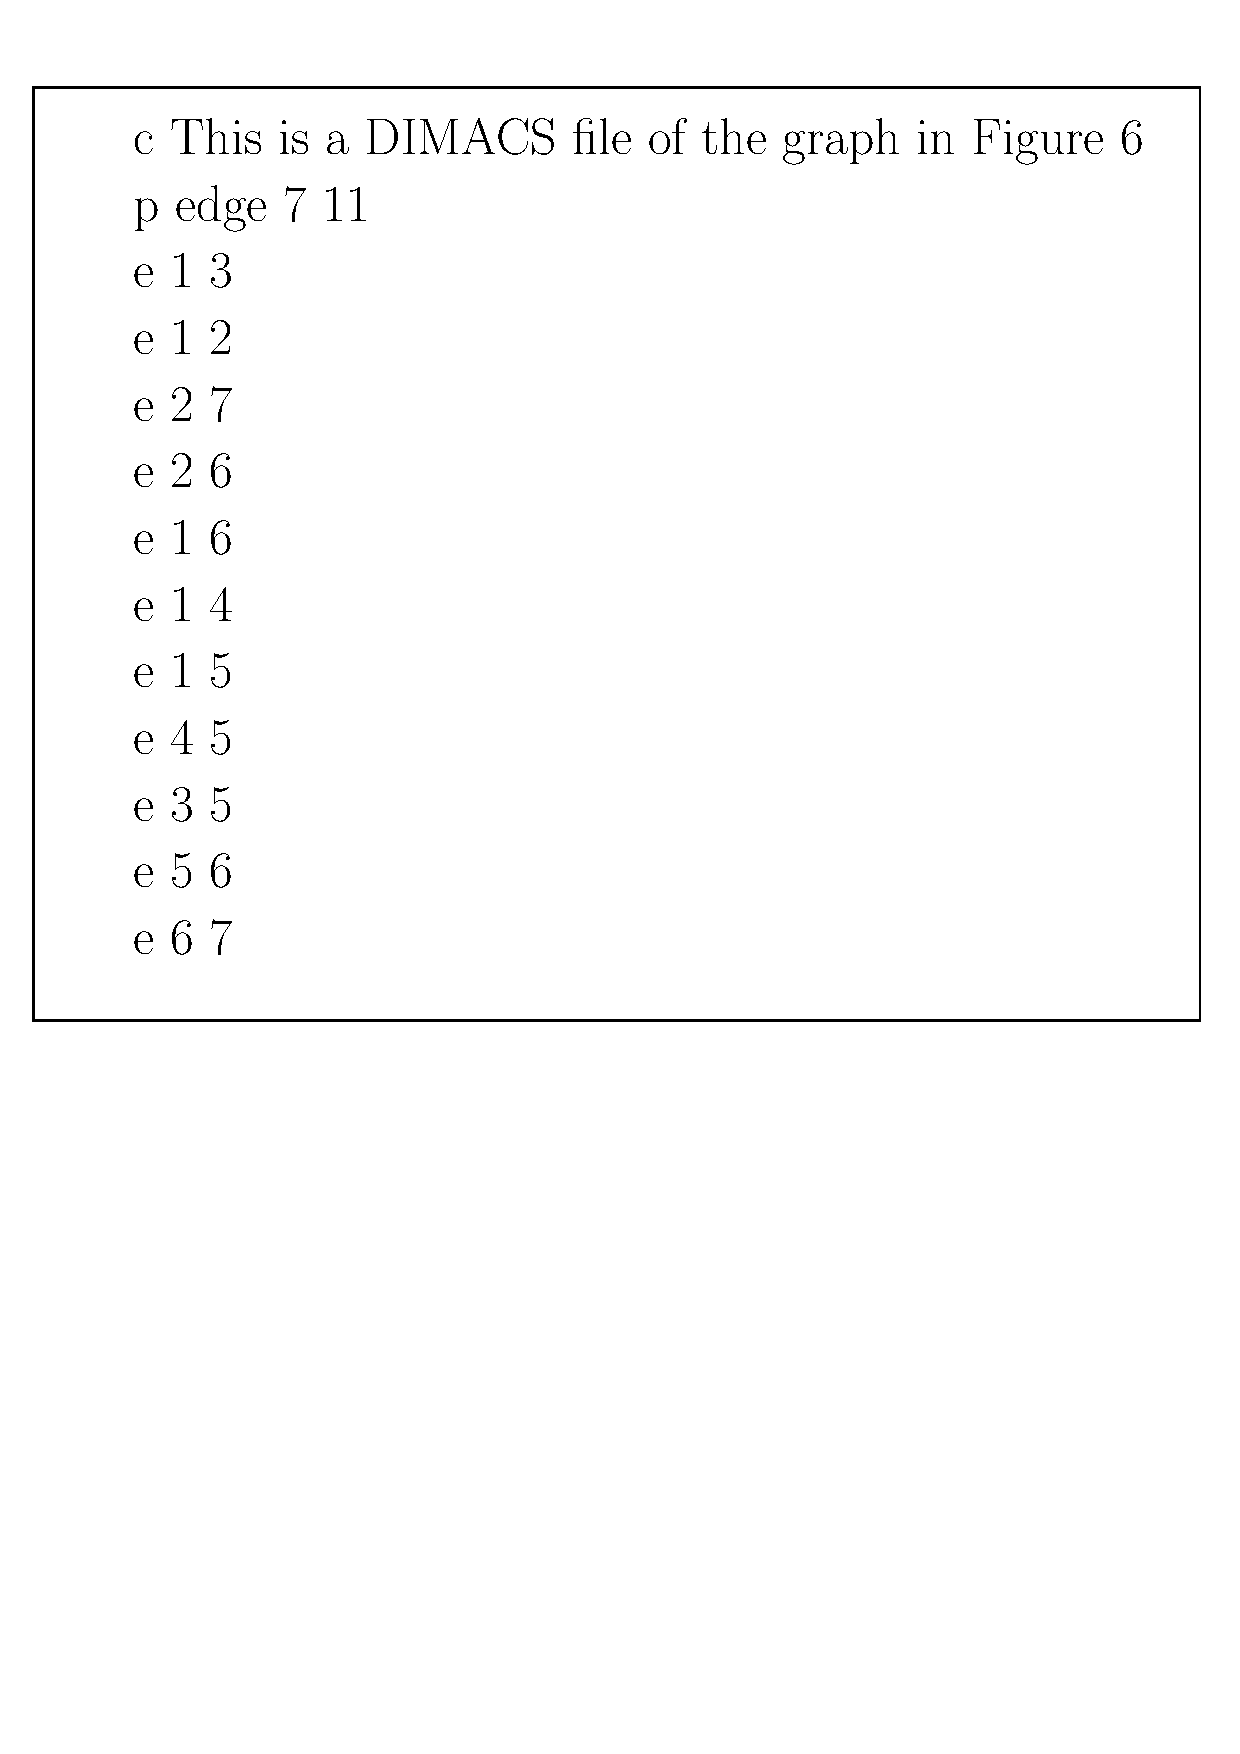
\includegraphics[scale = 0.5]{1/Dimacs.pdf}      \caption{A DIMACS file example of the problem in Figure \ref{Figure 6}}      \end{center} \end{figure}  
\subsection{Benchmarks}
\label{benchmark}
The benchmark instances used in experiments are the 180 uniform instances (unif) in random benchmark categories in SAT competition 2017  \cite{balyo2017proceedings}. In an unif problem file, all the clause have the same length.
The suffix 'k'  denotes the length of clauses. The r indicates the clause-to-variable ratio. The c and v are for the number of clauses and variables, while s is for the seed used in the generation process.
 Without flitering, there are at least 60 ( $33\%$ ) problems form our 180 benchmark collections are unsatisfiable.
\subsection{Used plots and tables}
the results of the following experiments are all shown in comparision table and  illusatrated in cactus plot.  \\
\\
\emph{\textbf{Comparison Table}}\\
See Table \ref{Experiment 1 Comparison Table} for example.\\
A comparison table compares the performance of different algorithms. The first column contains the 2-factor penalized runtime \footnote{Not like the PAR-2 scheme in SAT competition, we only  assign a 2-factor time limit penalization  for each unsolved benchmark which has been solved by another solver in the comparision.} of solving a set of benchmark problems. The fields of a comparison table in the following columns corresponds to the coloring sizes found with an algorithm.\\
\\
\emph{\textbf{Cactus Plot}}\\
See Figure \ref{Experiment 1 cactus plot} for an example.\\
A cactus plot shows the performance of different algorithms. The y-axis shows the time in second used to solve the benchmark graphs.  The y-axis is for the number of solved problems by a certain time. Each algorithm corresponds to a curve in different colors. The point $(u, v)$ on a curve means by $v$ seconds the corresponding algorithm have solved  $u$ problems.  \\

\subsection{Random seeds used in Experiments}
To make our experiments results reproducible and robust, we repeat our tests with three specific seeds. We produce the seeds in experiments as follows: First, we use the sum of characters of the name of the solver to seed the pseudo-random generator in c++.  Then we use this reinitialized generator to produce three random values, which are the seeds used later in our experiments. 
\begin{table}[h!]
%\begin{minipage}{\textwidth}                                                                                         
\begin{center}
    \begin{tabular}{|l|l|l|l|l|p{1cm}|}
\hline 
    solver&name&1.seed&2.seed&3.seed \\ \hline
	probSAT&probsat&1988822874&338954226 &858910419 \\ \hline
	yalSAT &yalsat&1851831967&280788293&1956345180 \\ \hline
	our local solver & local&1962042455&1112841915&566263966 \\ \hline
	our parallel solver & parallel &1749729997& 68910537& 473644167 \\ \hline
	
\end{tabular}
\caption[probSAT]{Parameter setting for competitor probSAT}
\end{center}
%\end{minipage}
\end{table} 
\subsubsection{Soft- and Hardware}
The single-threaded experiments were run on computers that had Two Intel Xeon E5-2683 v4 processors  (2.1 GHz 2x16-core + 2x16-HTcore) and 512GB RAM. The machine ran the 64-bit version
of  Ubuntu 14.04.5 LTS. 
\subsection{Parameter Settings in Experiment}
The $TimeOut$ is set to 5Minutes in the experiments of local searches.  For the probSAT heuristic, our local search uses the values for $c_b$ and $/epsilon$ suggested in the probSAT paper.  The $tolerence$ $ \tau$ used in the experiments is generated with the help of the algorithm parameter optimization tool SMAC [29] (sequential model-based algorithm configuration). SMAC ran our algorithms on LARGE problems in the UNIF category in SAT 2012 ($75\%$ of the instances training instances,  $25\%$ as test instances) using different   $ \tau \in [0, 10]$\footnote{Because of high time consume in parameter optimation, we solely compare $\tau$  as a natural number form One to Ten.}  and randomly generated seeds. With the help of SMAC.


\subsection{Experiments}
\subsubsection{Experiment 1: initAssign(F)}
Experiment 1 compares two three strategies of initialization in our solver. The $biasInit$ suggestion is assign variables based on occurrences of their literals. It assigns True to variables whose positive literal occurs more than its negative literal. Another alternative $randomInit$ is to build a coloring randomly. In a combination of these two variants $randomBiasInit$, the boolean value is assigned to variables based on bias randomly on literals occurrences. the probability to assign True to variable $v_i$ is $\frac{posOccurences[i]}{posOccurences[i]+negOccurences[i]}$. \\
\begin{table}[H]
%\begin{minipage}{\textwidth}                                                                                         
\begin{center}
    \begin{tabular}{|l|l|l|l|p{1cm}|}
\hline 
    k &$RandomInit$&$BiasInit$&$Bias$-$RandomInit$ \\ \hline
	3&9221.9 (\textbf{55})&9157.76 (54)&\textbf{ 9078.27}(\textbf{55}) \\ \hline
	5&7143.9 (82)&\textbf{4351.09}(\textbf{87})&4582.54 (\textbf{87})\\ \hline

	7& 	6238.51(60)&\textbf{5421.9} (60)& 6310.7(60)\\ \hline
	
\end{tabular}
\end{center}
%\end{minipage}
\end{table} 

\begin{figure}[H]
\begin{center}
  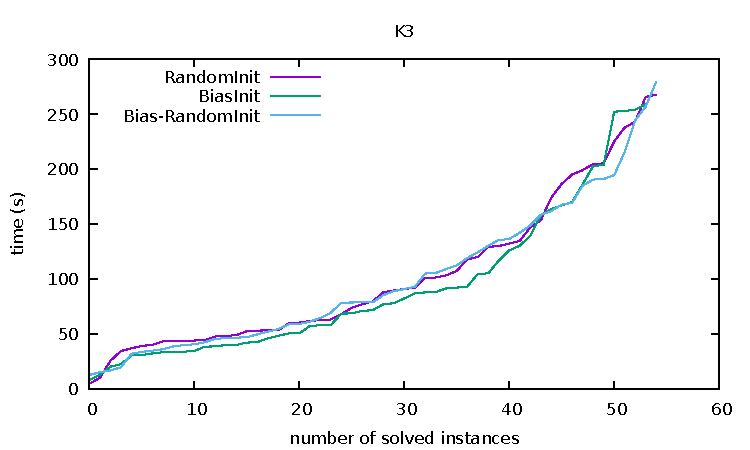
\includegraphics[scale = 1]{DATA/K3/e1.pdf}
  \end{center}
  \caption{Three suggestions have very similar performance.}
  \label{Experiment 1 k3 cactus plot}
  \end{figure}
  \begin{figure}[H]
\begin{center}
  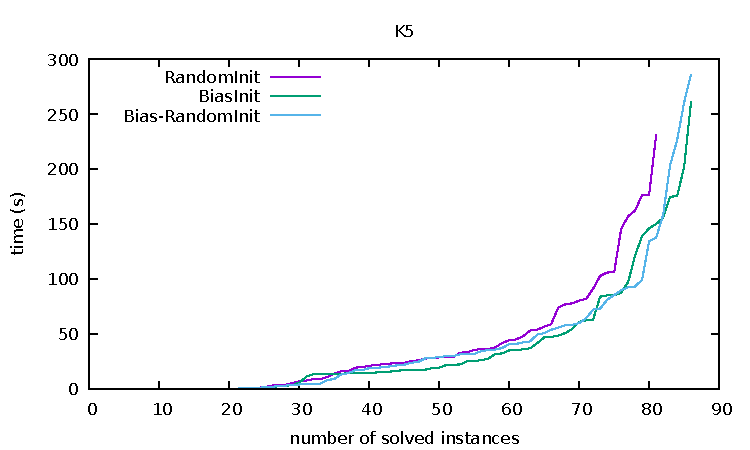
\includegraphics[scale = 1]{DATA/K5/e1.pdf}
  \end{center}
  \caption{Two bias suggestions show advantages especially for huge instances.}
  \label{Experiment 1 k5 cactus plot}
  \end{figure}
  \begin{figure}[H]
\begin{center}
  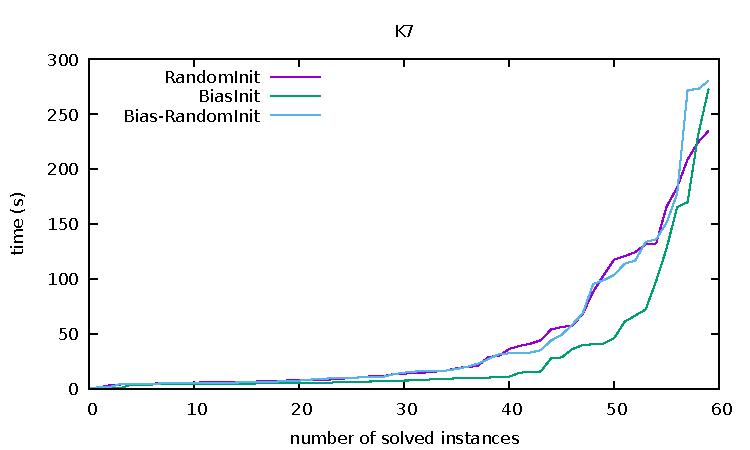
\includegraphics[scale = 1]{DATA/K7/e1.pdf}
  \end{center}
  \caption{For 7SAT problems, the two random Initialization are similar in performance, while the bias initialization shows its efficiency.}
  \label{Experiment 1 k7 cactus plot}
  \end{figure}
  \clearpage
\subsubsection{Experiment 2: pickVar(F)}  
With the comparison of three Variant of $pickVal$ with the one in probSAT, our suggestions are faster and solve more instances in K3 and K5.  For K7,  there are no noticeable differences in results.
\begin{table}[h!]
%\begin{minipage}{\textwidth}                                                                                         
\begin{center}
    \begin{tabular}{|l|l|l|l|p{3cm}|}
\hline 
    k &$probSAT$&$WALK$&$Average$&$Random-Flip$ \\ \hline
	3&9221.9 (55)&7430.12 (57)&\textbf{6161.11}(\textbf{61})&8362.42 (55) \\ \hline
	5&7143.9 (82)&4433.05 (87)&\textbf{3308.16}(\textbf{89})&4052.47(87)\\ \hline

	7& 	6238.51(\textbf{60})& 6358.76(\textbf{60})&6525.597(59)&\textbf{5800.46}(\textbf{60})\\ \hline
	
\end{tabular}
\end{center}
%\end{minipage}
\end{table} 

\begin{figure}[H]
\begin{center}
  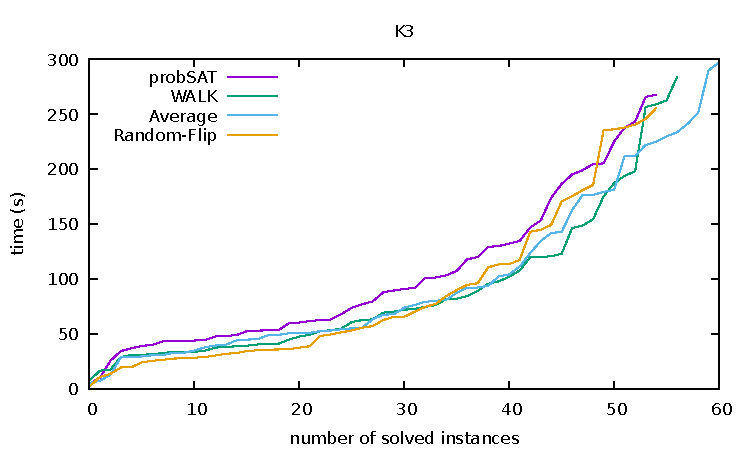
\includegraphics[scale = 1]{DATA/K3/e2.pdf}
  \end{center}
  \caption{Three suggestions have very similar performance.}
  \label{Experiment 2 k3 cactus plot}
  \end{figure}
  \begin{figure}[H]
\begin{center}
  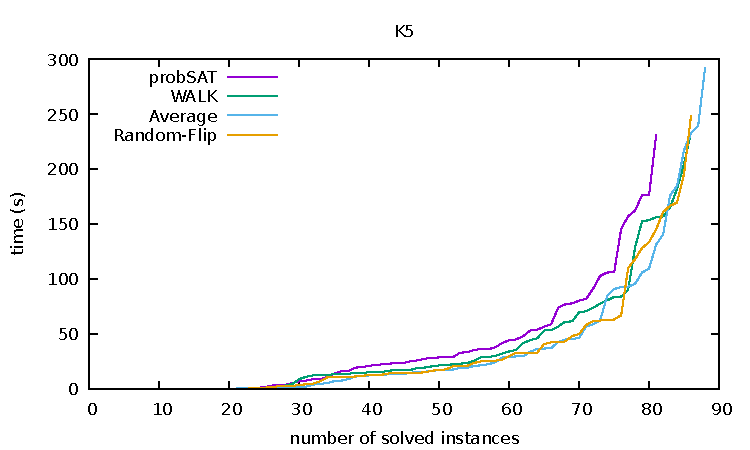
\includegraphics[scale = 1]{DATA/K5/e2.pdf}
  \end{center}
  \caption{Two bias suggestions show advantages especially for huge instances.}
  \label{Experiment 2 k5 cactus plot}
  \end{figure}
  \begin{figure}[H]
\begin{center}
  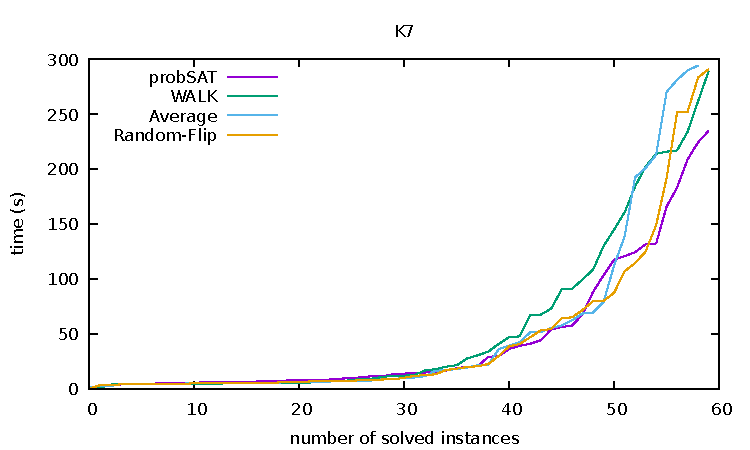
\includegraphics[scale = 1]{DATA/K7/e2.pdf}
  \end{center}
  \caption{For 7SAT problems, the two random Initialization are similar in performance, while the bias initialization shows its efficiency.}
  \label{Experiment 2 k7 cactus plot}
  \end{figure}

\subsubsection{Experiment 3: WALK with Simulated Annealing} 
\begin{table}[H]
%begin{minipage}{\textwidth}                                                                                         
\begin{center}
    \begin{tabular}{|l|l|l|l|p{3cm}|}
\hline 

    k &$WALK$&$WALK-Local$&$WALK-Global$ \\ \hline      
    3 &\textbf{7430.12}(\textbf{57})&	8346.76(56)	&9023.96(56)  \\ \hline
    5&4433.05(87)	&3330.61(89)	&\textbf{3117.45}(\textbf{89}) \\ \hline
    7&6358.76(60)	&\textbf{5409.67}(\textbf{61})&	6566.06(59) \\ \hline	
\end{tabular}
\end{center}
%\end{minipage}
\end{table} 

\begin{figure}[H]
\begin{center}
  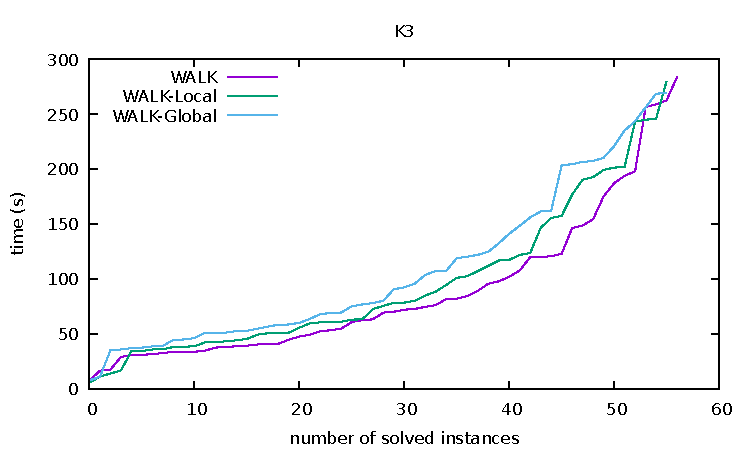
\includegraphics[scale = 1]{DATA/K3/e3w.pdf}
  \end{center}
  \caption{Three suggestions have very similar performance.}
  \label{Experiment 3 k3-w cactus plot}
  \end{figure}
  \begin{figure}[H]
\begin{center}
  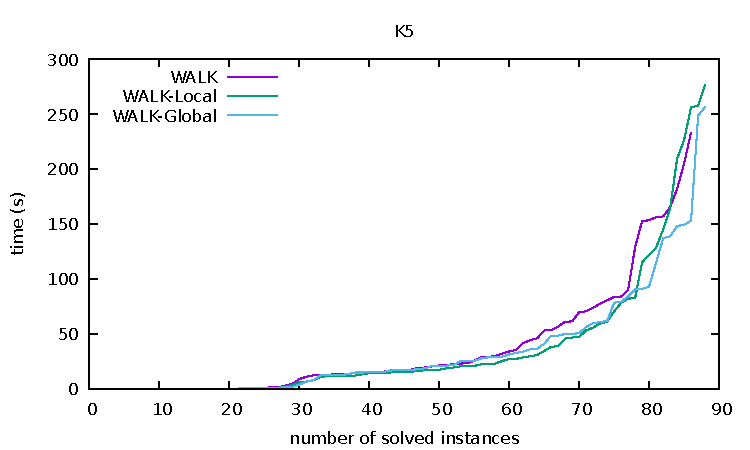
\includegraphics[scale = 1]{DATA/K5/e3w.pdf}
  \end{center}
  \caption{Two bias suggestions show advantages especially for huge instances.}
  \label{Experiment 3 k5-w cactus plot}
  \end{figure}
  \begin{figure}[H]
\begin{center}
  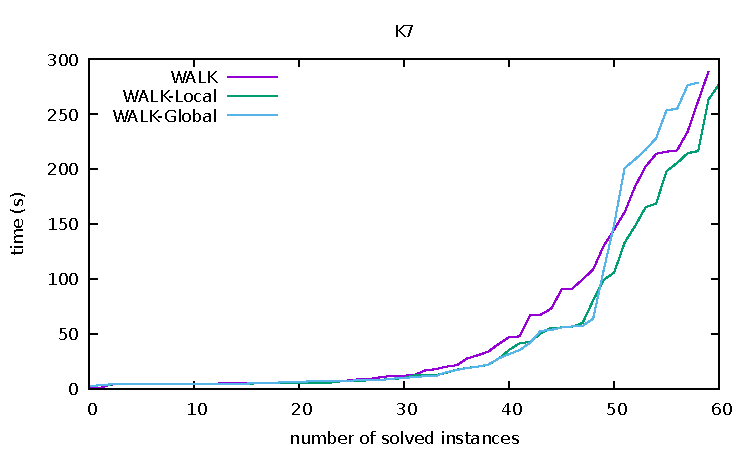
\includegraphics[scale = 1]{DATA/K7/e3w.pdf}
  \end{center}
  \caption{For 7SAT problems, the two random Initialization are similar in performance, while the bias initialization shows its efficiency.}
  \label{Experiment 3 k7-w cactus plot}
  \end{figure}
\subsubsection{Experiment 4: Average with Simulated Annealing} 
\begin{table}[h!]
%\begin{minipage}{\textwidth}                                                                                         
\begin{center}
    \begin{tabular}{|l|l|l|l|p{3cm}|}
\hline 

    k &$Average$&$Average-Local$&$WALK-Global$ \\ \hline      
    3 & \textbf{6161.11}(\textbf{61})	&9254.18(53)&	9870.25(53) \\ \hline
    5& 3308.16(89)	&\textbf{2793.32}(89)&	2939.74(89)\\ \hline
    7& 6525.59(59)&\textbf{	3829.95}(\textbf{65})	&5738.2(61)\\ \hline	
\end{tabular}
\end{center}
%\end{minipage}
\end{table} 

  \begin{figure}[H]
\begin{center}
  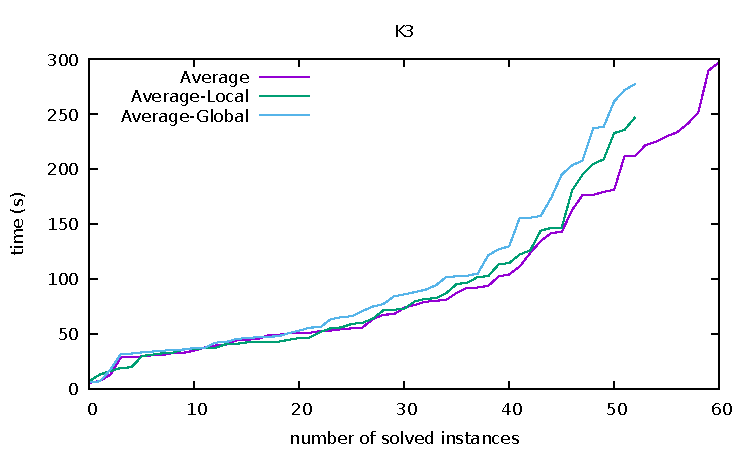
\includegraphics[scale = 1]{DATA/K3/e3a.pdf}
  \end{center}
  \caption{Three suggestions have very similar performance.}
  \label{Experiment 4 k3 cactus plot}
  \end{figure}
  \begin{figure}[H]
\begin{center}
  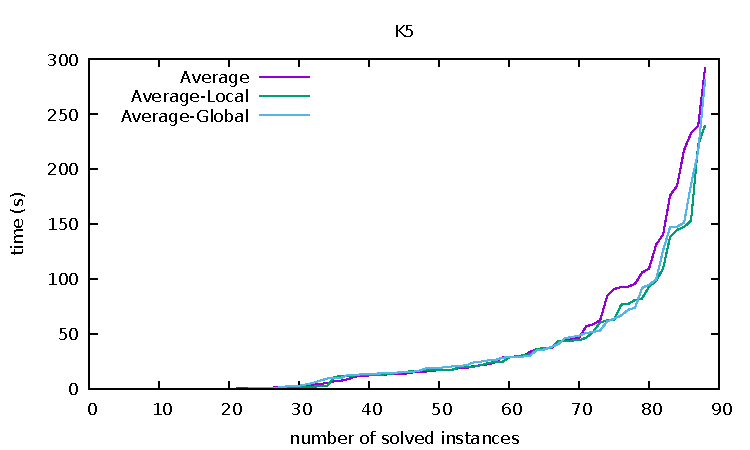
\includegraphics[scale = 1]{DATA/K5/e3a.pdf}
  \end{center}
  \caption{Two bias suggestions show advantages especially for huge instances.}
  \label{Experiment 4 k5 cactus plot}
  \end{figure}
  \begin{figure}[H]
\begin{center}
  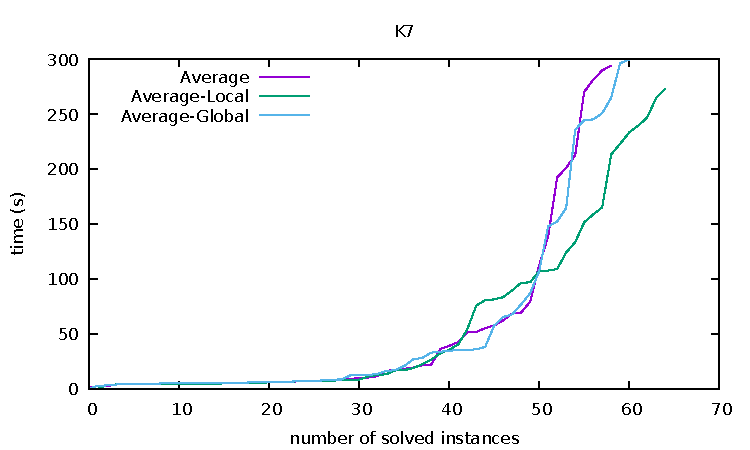
\includegraphics[scale = 1]{DATA/K7/e3a.pdf}
  \end{center}
  \caption{For 7SAT problems, the two random Initialization are similar in performance, while the bias initialization shows its efficiency.}
  \label{Experiment 4 k7 cactus plot}
  \end{figure}
\subsubsection{Experiment 5: Random-Flip with Simulated Annealing} 
  \begin{table}[H]
%\begin{minipage}{\textwidth}                                                                                         
\begin{center}
    \begin{tabular}{|l|l|l|l|p{3cm}|}
\hline 

    k &$Random-Flip$&$Random-Flip-Local$&$Random-Flip-Global$ \\ \hline      
    3 &  8362.42(55)&8409.8(55)	&\textbf{7308.01}(\textbf{58})\\ \hline
    5&4052.47(87)&	4132.07(87)&\textbf{4003.06}(\textbf{88}) \\ \hline
    7& 5800.46(60) &6792.23(59) &	\textbf{4903.61}(\textbf{60})\\ \hline
	
\end{tabular}
\end{center}
%\end{minipage}
\end{table}
  \begin{figure}[H]
\begin{center}
  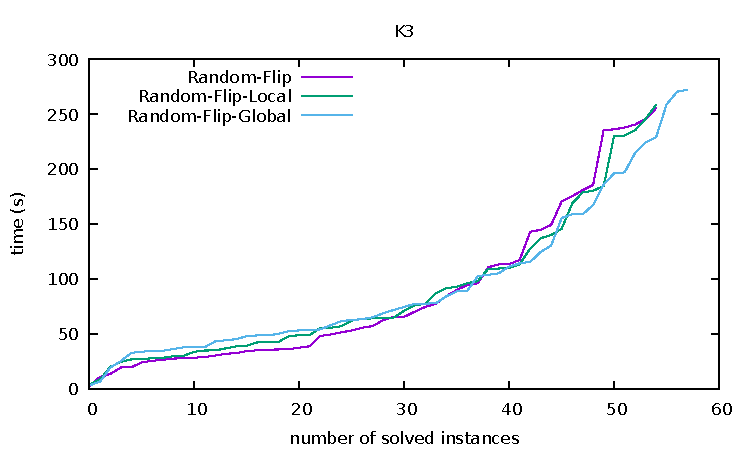
\includegraphics[scale = 1]{DATA/K3/e3r.pdf}
  \end{center}
  \caption{Three suggestions have very similar performance.}
  \label{Experiment 5 k3 cactus plot}
  \end{figure}
  \begin{figure}[H]
\begin{center}
  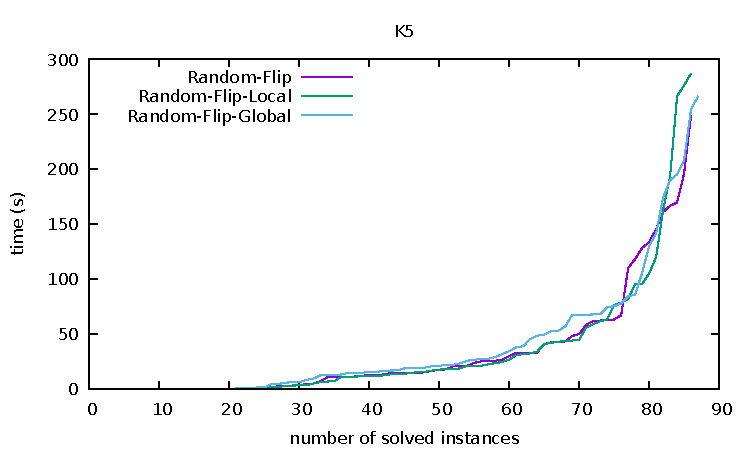
\includegraphics[scale = 1]{DATA/K5/e3r.pdf}
  \end{center}
  \caption{Two bias suggestions show advantages especially for huge instances.}
  \label{Experiment 5 k5 cactus plot} 
  \end{figure}
  \begin{figure}[H]
\begin{center}
  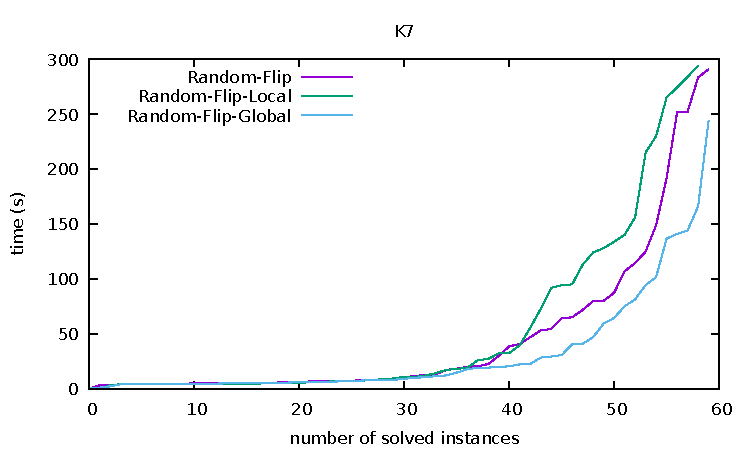
\includegraphics[scale = 1]{DATA/K7/e3r.pdf}
  \end{center}
  \caption{For 7SAT problems, the two random Initialization are similar in performance, while the bias initialization shows its efficiency.}
  \label{Experiment 5 k7 cactus plot}
  \end{figure}
\subsubsection{Experiment 6: probSAT vs WALK.}  
  \begin{figure}[H]
\begin{center}
  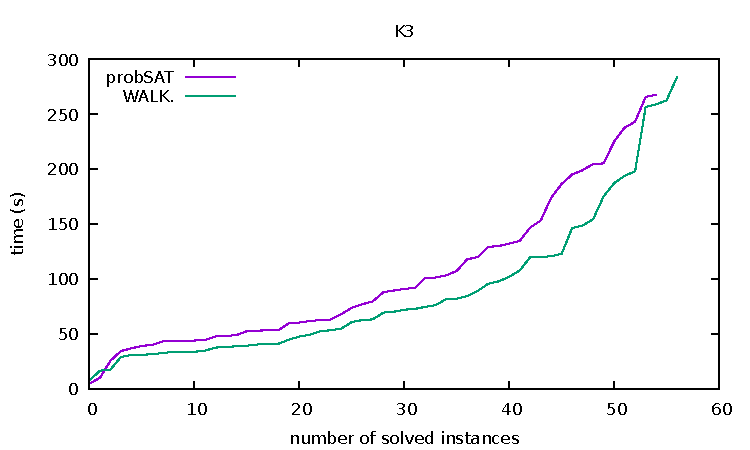
\includegraphics[scale = 1]{DATA/K3/e4w.pdf}
  \end{center}
  \caption{Three suggestions have very similar performance.}
  \label{Experiment 6 k3 cactus plot}
  \end{figure}
  \begin{figure}[H]
\begin{center}
  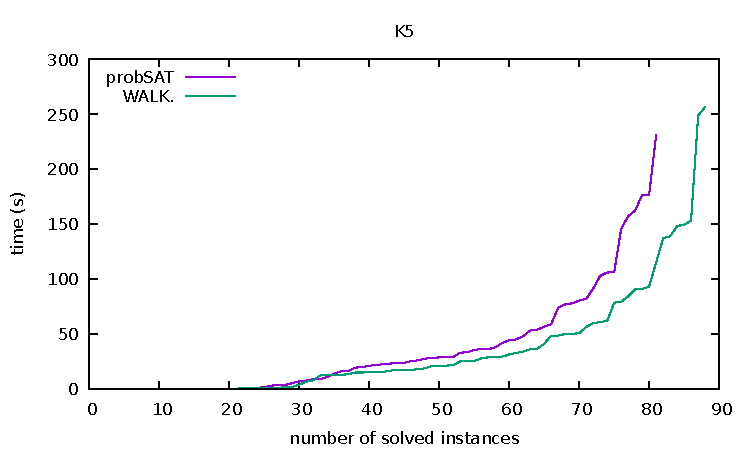
\includegraphics[scale = 1]{DATA/K5/e4w.pdf}
  \end{center}
  \caption{Two bias suggestions show advantages especially for huge instances.}
  \label{Experiment 6 k5 cactus plot}
  \end{figure}
  \begin{figure}[H]
\begin{center}
  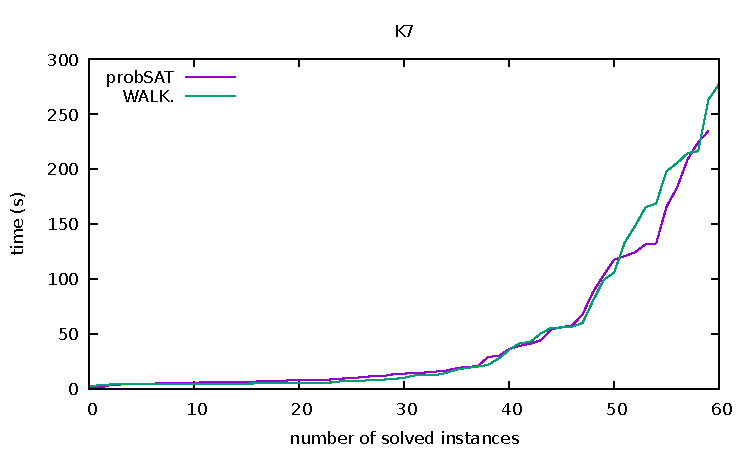
\includegraphics[scale = 1]{DATA/K7/e4w.pdf}
  \end{center}
  \caption{For 7SAT problems, the two random Initialization are similar in performance, while the bias initialization shows its efficiency.}
  \label{Experiment 7 k7 cactus plot}
  \end{figure}

\subsubsection{Experiment 7: probSAT vs Average.}   
  \begin{figure}[H]
\begin{center}
  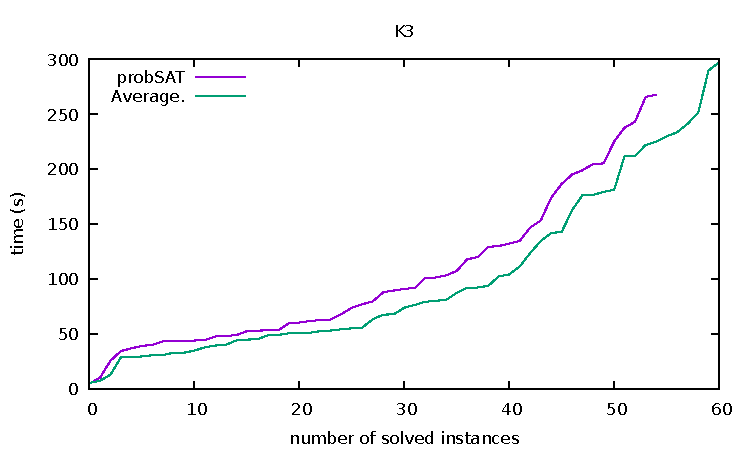
\includegraphics[scale = 1]{DATA/K3/e4a.pdf}
  \end{center}
  \caption{Three suggestions have very similar performance.}
  \label{Experiment 7 k3 cactus plot}
  \end{figure}
  \begin{figure}[H]
\begin{center}
  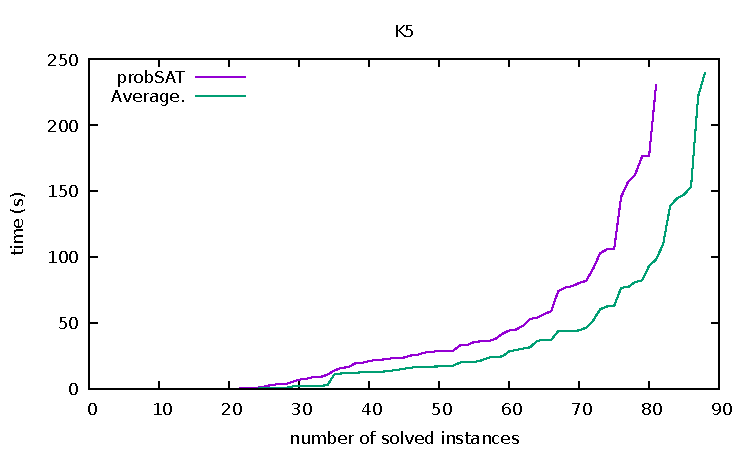
\includegraphics[scale = 1]{DATA/K5/e4a.pdf}
  \end{center}
  \caption{Two bias suggestions show advantages especially for huge instances.}
  \label{Experiment 7 k5 cactus plot}
  \end{figure}
  \begin{figure}[H]
\begin{center}
  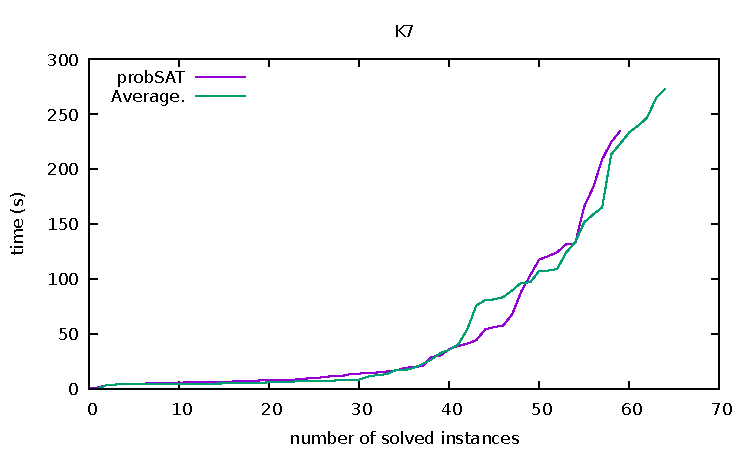
\includegraphics[scale = 1]{DATA/K7/e4a.pdf}
  \end{center}
  \caption{For 7SAT problems, the two random Initialization are similar in performance, while the bias initialization shows its efficiency.}
  \label{Experiment 7 k7 cactus plot}
  \end{figure}
\subsubsection{Experiment 8:probSAT vs Random-Flip.}  
  \begin{figure}[H]
\begin{center}
  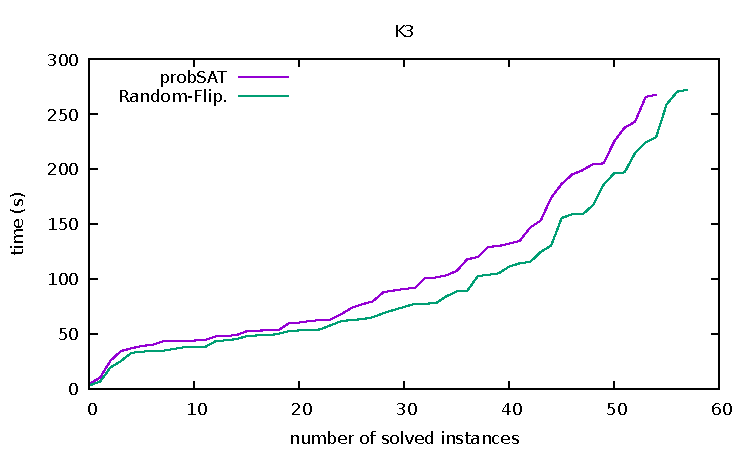
\includegraphics[scale = 1]{DATA/K3/e4r.pdf}
  \end{center}
  \caption{Three suggestions have very similar performance.}
  \label{Experiment 8 k3 cactus plot}
  \end{figure}
  \begin{figure}[H]
\begin{center}
  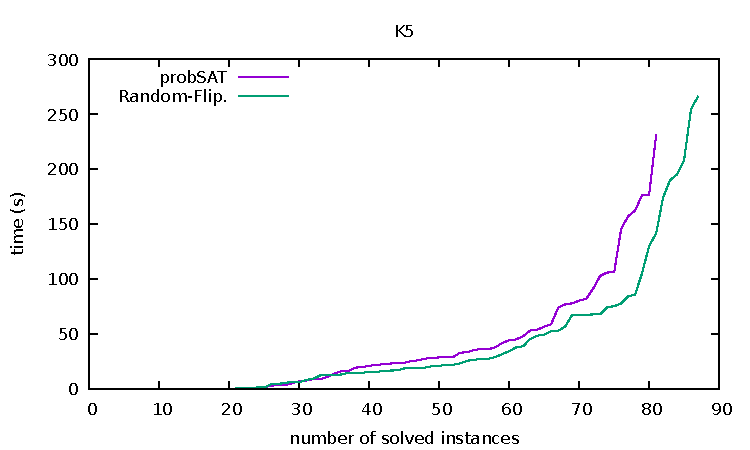
\includegraphics[scale = 1]{DATA/K5/e4r.pdf}
  \end{center}
  \caption{Two bias suggestions show advantages especially for huge instances.}
  \label{Experiment 8 k5 cactus plot}
  \end{figure}
  \begin{figure}[H]
\begin{center}
  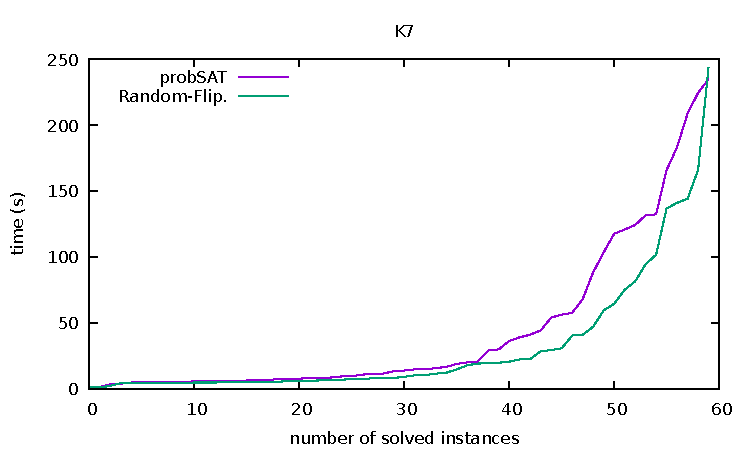
\includegraphics[scale = 1]{DATA/K7/e4r.pdf}
  \end{center}
  \caption{For 7SAT problems, the two random Initialization are similar in performance, while the bias initialization shows its efficiency.}
  \label{Experiment 8 k7 cactus plot}
  \end{figure} 
\subsubsection{Experiment 9: 2017-UNIF Comparision} 
   \begin{table}[H]
%\begin{minipage}{\textwidth}                                                                                         
\begin{center}
    \begin{tabular}{|l|l|l|l|l|p{3cm}|}
\hline 

    k &$probSAT$&$yalSAT$&$WALK$&$Average$/$swpSAT$&$Random-Flip$ \\ \hline      
    3 &9221.9(55)&17062.35(41)&7430.12(57)&\textbf{6161.11}(\textbf{61})&7308.01(58)\\ \hline
    5& 7143.9(82)&5676.63(85)&3330.61(89)&\textbf{2939.74}(\textbf{89})&4003.06(88)\\ \hline
    7& 6238.51(60)&10063.4(54)&5409.67(61)&\textbf{3829.95}(\textbf{65})&4903.61(60)\\ \hline
	
\end{tabular}
\end{center}
%\end{minipage}
\end{table}
  \begin{figure}[H]
\begin{center}
  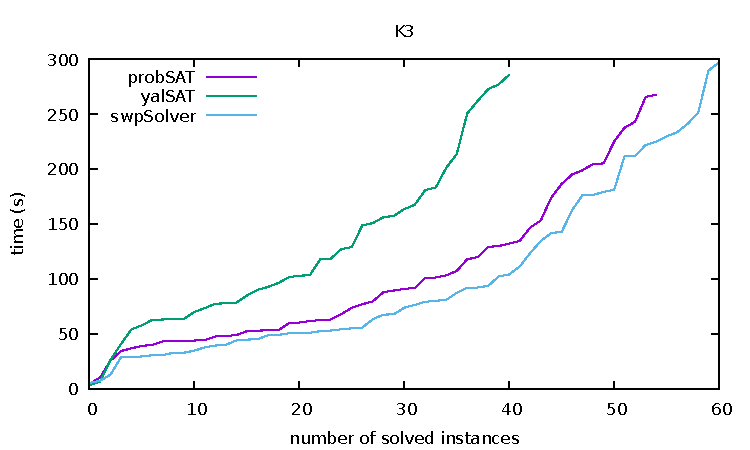
\includegraphics[scale = 1]{DATA/K3/e5.pdf}
  \end{center}
  \caption{Three suggestions have very similar performance.}
  \label{Experiment 9 k3 cactus plot}
  \end{figure}
  \begin{figure}[H]
\begin{center}
  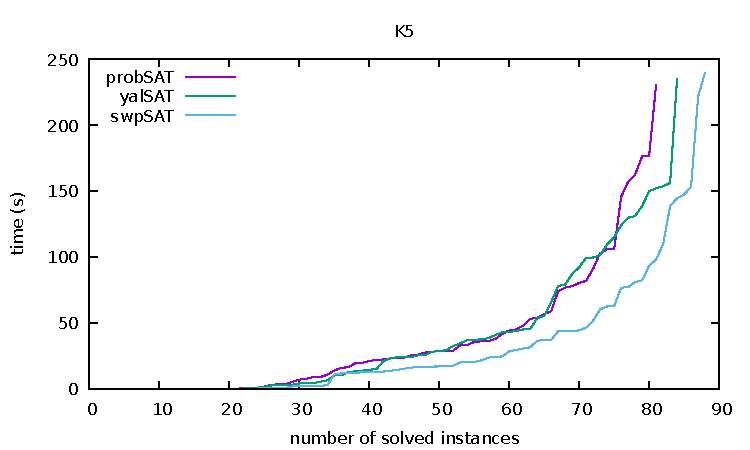
\includegraphics[scale = 1]{DATA/K5/e5.pdf}
  \end{center}
  \caption{Two bias suggestions show advantages especially for huge instances.}
  \label{Experiment 9 k5 cactus plot}
  \end{figure}
  \begin{figure}[H]
\begin{center}
  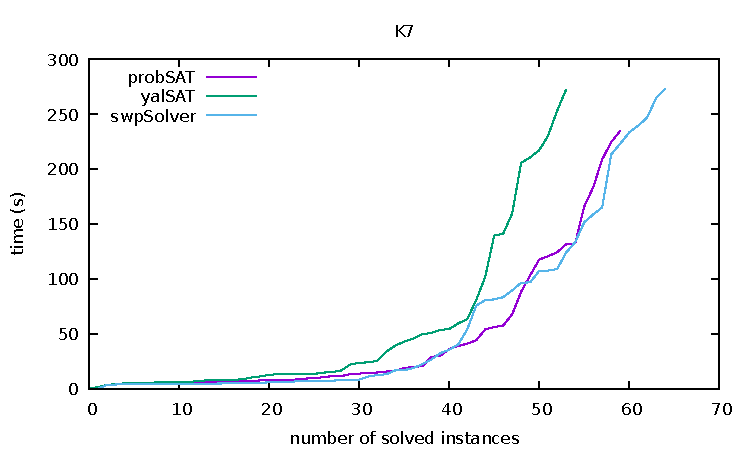
\includegraphics[scale = 1]{DATA/K7/e5.pdf}
  \end{center}
  \caption{For 7SAT problems, the two random Initialization are similar in performance, while the bias initialization shows its efficiency.}
  \label{Experiment 9 k7 cactus plot}
  \end{figure} 
  \begin{figure}[H]
\begin{center}
  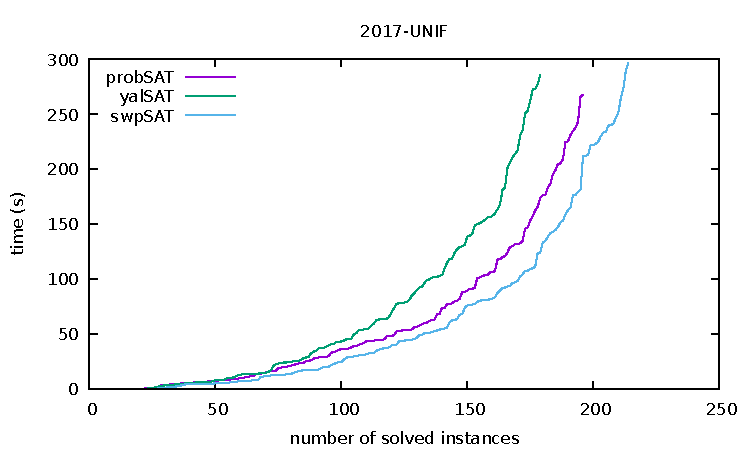
\includegraphics[scale = 1]{DATA/UNIF/e5.pdf}
  \end{center}
  \caption{For 7SAT problems, the two random Initialization are similar in performance, while the bias initialization shows its efficiency.}
  \label{Experiment 9 all cactus plot}
  \end{figure} 
\subsubsection{Experiment 10: 2009-UNIF Comparision} 

TODO: get the results of new version on 132 (still occupied by some guy)

  
\section{Conclusion}
\label{sec:conc}
\subsection{Further work}
\section{Bibliography}
\bibliographystyle{ieeetr}
\bibliography{references}
\end{document}
